\chapter[Diversion Detection]{Diversion Detection}

The second aspect of this work identifies locations sensitive to diversion in a generic pyroprocessing facility. This work leverages two approaches: applying
a cumulative sum detection algorithm and performing sensitivity analysis on key facility parameters. 
\section{Cumulative Sum}

\subsection{Requirements of Diversion Detection}


The cumulative sum method (CUSUM) applied to Pyre was chosen to fit the following requirements: function with minimal prior information, have online diversion detection
capabilities, and fit a modular approach. The CUSUM change detection algorithm calculates expected mean value of an observed data stream as shown by the following equations \cite{basseville_detection_1993}.

\begin{align}
	f_{t+1} &= max(0, f_t + x_t - \mu - \delta) \\
	\intertext{Where}
	x_t &= \mbox{observed data at time t} \nonumber \\
	\mu &= \mbox{approximated mean of x} \nonumber \\
	\delta &= \mbox{acceptable change} \nonumber
\end{align}

This general function adds new observed values to the calculated mean. If the value is within a region of allowable change, typically 3$\sigma$, the change is not reported. 
We favor this online diversion detection capability in an effort to achieve timely detection goals set by the IAEA \cite{international_atomic_energy_agency_implications_2004}.
These intermittent inspections only have access to portions of the complete data stream, thus we aim to mimic reality as closely as possible. In addition, we need this
algorithm to work on a variety of facilities with various active sub-processes.

\subsection{Limitations of selected method}

The CUSUM approach is not without its drawbacks: since there is no prior data assumed we must generate a reasonable mean from observed data before being able to detect diversion. In this work
we assume a startup time of approximately 6 months before an appropriate mean can be developed. The next limitation faced with this approach is that CUSUM assumes one can only observe one data stream at a time, while
real inspections take a wide range of conditions into account. This concern is addressed by using sensitivity analysis, as seen later in this chapter, to inform on the most crucial
sub-processes or settings. 

CUSUM relies on a variable mean and noise to obscure possible change points. When a simulator knows the exact value at each time step, without human reporting or measurement error, change 
detection becomes trivial. To best represent the uncertainty inherent in material accountancy measurement, noise is artificially created when the CUSUM class reads data. This way \Cyclus retains its constant operating value while the change point
has potential to be obscured by measurement error. These detector uncertainties are assumed from common non-destructive and destructive assay practices used by the SEE LANL safeguards training course \cite{root_see_2019}.

\section{Verification}

To test operator diversion capabilities, we ran the EG01-EG24 transition scenario shown in chapter 3 with inside operators. The scenario described in Table \ref{tab:setup} contains an LWR and SFR configuration for Pyre. Each prototype siphoned material with different quantities and frequencies to demonstrate its reconfigurability. The pyroprocessing facility that exclusively accepts LWR fuel siphoned off 5\% every 10 timesteps while the facility that only accepts SFR fuel siphoned off 1\% excess every other timestep.  Results for this scenario are shown in Figure \ref{fig:divertmat}.

\begin{figure}
	\centering
	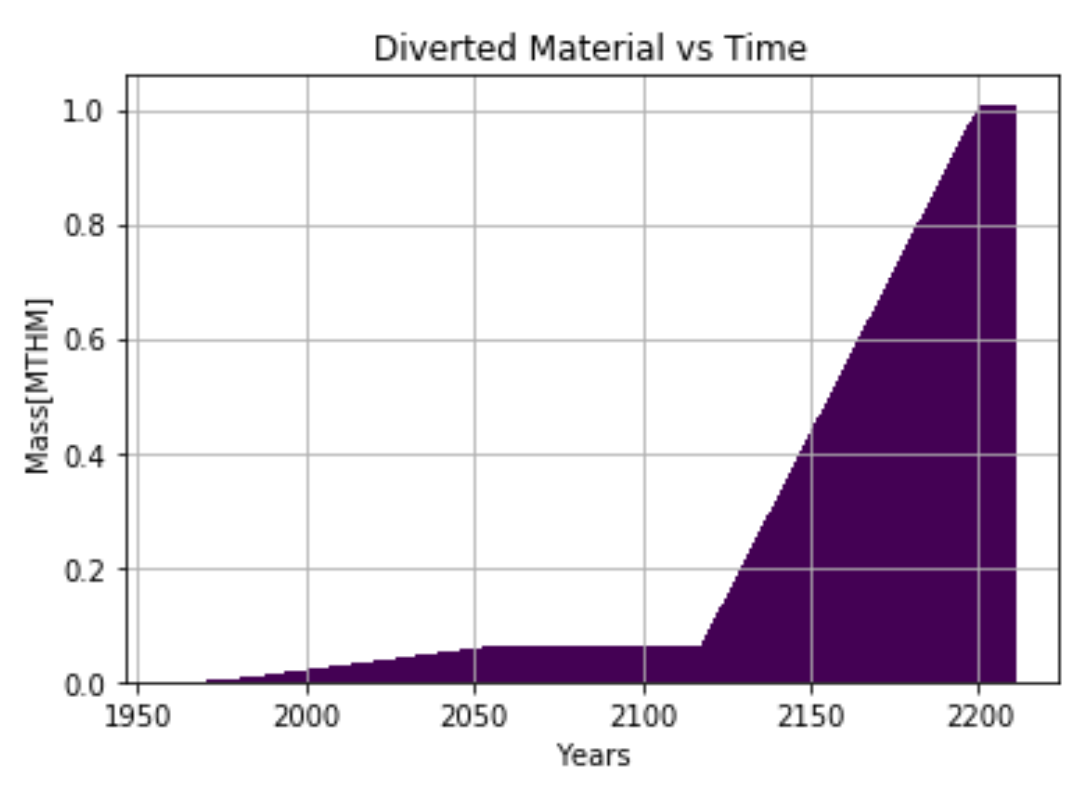
\includegraphics[width=0.9\linewidth]{images/divertmat}
	\caption{A timeseries of diverted material from transition scenario EG01-EG24.}
	\label{fig:divertmat}
\end{figure}

\section{Sensitivity Analysis}

The sensitivity analysis approach in this work illuminates the limits of monitoring future pyroprocessing facilities. This work relies on Dakota to alter \Cyclus input files and provides a number of statistics packages, allowing us to easily
run batches of scenarios. To properly use Dakota with \Cyclus, we must use DCWrapper, which uses python to interface between Dakota and \Cyclus' xml input files. 
Key parameters were sampled over a range of values for diversion to verify the archetype's capabilities and identify operational ranges. The range for each parameter is shown in Table \ref{tab:range}. 

\begin{table}[h]
	\centering
	\begin{tabularx}{0.85\linewidth}{lccc}
		\hline
		\textbf{Parameter} & \textbf{Lower Bound} & \textbf{Upper Bound} & \textbf{Units} \\
		\hline \hline
		Electrorefiner Temp & 750 & 1000 & $^\circ C$ \\ \hline
		Electrorefiner Pressure & 100 & 760 & mTorr \\ \hline
		Electrorefiner Stirrer Speed & 0 & 100 & rpm \\ \hline
		Electrowinner Current & 5 & 10 & Amps \\ \hline
		Electrowinner Flow Rate & 2 & 4.5 & cm/s \\ \hline
		Electrowinner Process Time & 1 & 4 & hours \\ \hline
	\end{tabularx}
	\caption {Range of Each Sensitivity Analysis Parameter Sample.}
	\label {tab:range}
\end{table}

Parameters were selected from the most attractive
sub-processes for diversion, the electrorefiner and electrowinner. These two processes are responsible for the production of Uranium and U/TRU ingots, therefore sensitivity analysis was run
on each of their key parameters: Temperature, Current, Flowrate, Pressure, Stirrer Speed, and Reprocessing Time. Six samples were selected at regular intervals across the range of each parameter. For each setting we observe how much material can be diverted within a month.

\subsection{Electrorefiner Temperature}

The first setting for consideration is the electrorefiner's temperature. As discussed in methodology, the range for this setting is 500 to 1000 $^\circ C$ with typical operation above 750 $^\circ C$. These values can be seen isotopically in Figure \ref{fig:ref-temp-sa}.
The 750 $^\circ C$ stream is then subtracted from the sampled streams to determine the impact of increasing temperature on divertable material.
While temperature is a key aspect to the electrorefiner, Figure \ref{fig:ref-temp-diff} shows that temperatures approaching 1000 $^\circ C$ result in diminishing returns.

\begin{figure}
	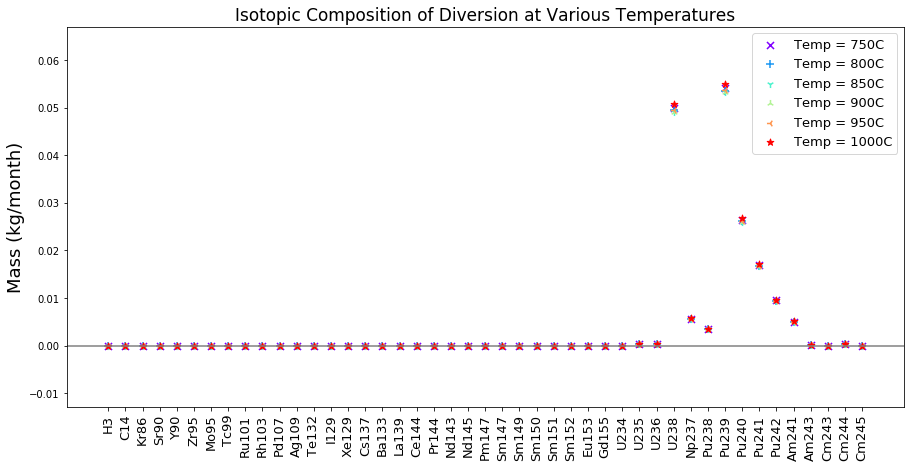
\includegraphics[width=\linewidth]{images/temperature-sa-comp}
	\caption{Isotopic composition of the diverted material stream at various electrorefiner temperatures.}
	\label{fig:ref-temp-sa}
\end{figure}

\begin{figure}
	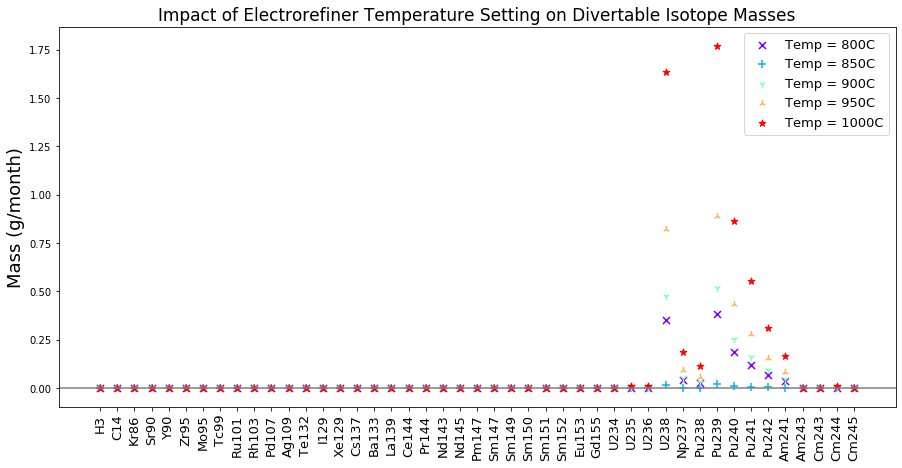
\includegraphics[width=\linewidth]{images/temperature-sa-diff}
	\caption{Isotopic composition of the diverted material stream at various electrorefiner temperatures.}
	\label{fig:ref-temp-diff}
\end{figure}

\subsection{Electrorefiner Pressure}

Available in advanced electrorefiners, lower vacuum pressure can improve separation efficiency as well. Similar to our analysis of temperature, isotopic compositions of
divertable material can be seen in Figure \ref{fig:ref-press-sa}. Our baseline for the comparison is atmospheric pressure as this will represent facilities lacking this
functionality. 

\begin{figure}
	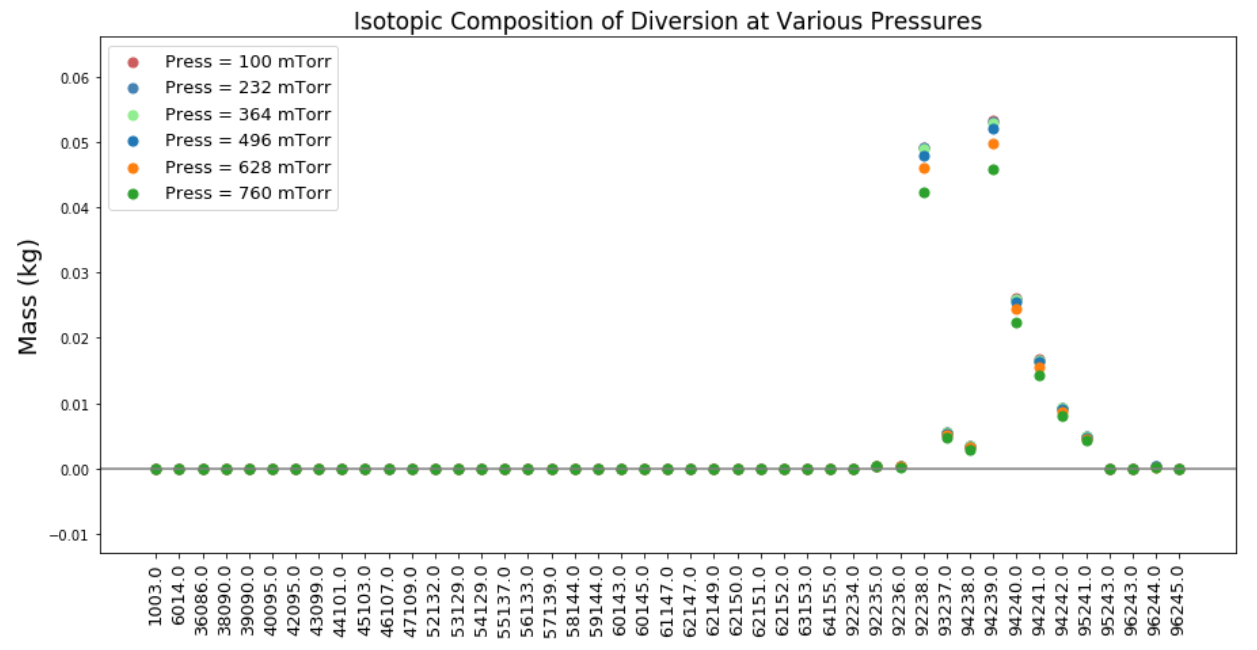
\includegraphics[width=\linewidth]{images/pressure-sa-comp}
	\caption{Isotopic composition of the Diverted material stream at various electrorefiner pressures.}
	\label{fig:ref-press-sa}
\end{figure}

\begin{figure}
	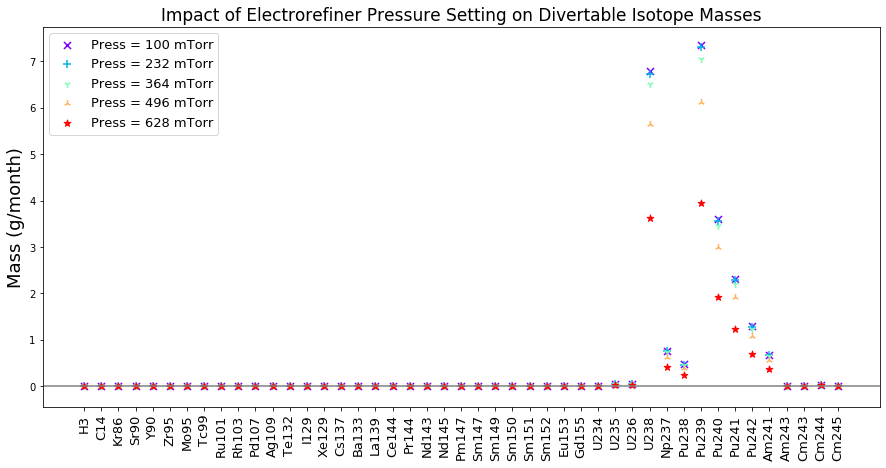
\includegraphics[width=\linewidth]{images/pressure-sa-diff}
	\caption{Isotopic composition of the Diverted material stream at various electrorefiner pressures.}
	\label{fig:ref-press-diff}
\end{figure}

\subsection{Electrorefiner Stirrer Speed}

The central stirrer is another setting particular to advanced refining techniques \cite{lee_advanced_2008}. Pyre tracks this parameter since adding a stirrer to processes can be a simple procedure. Figure \ref{fig:ref-rot-sa} shows the isotopic distribution associated with a
range of different stirrer speeds. Stirrer speed higher than 100 rpm results in uranium dendrites returning
to the salt. Therefore, in Figure \ref{fig:ref-rot-diff} this work took 0 rpm as our baseline to represent facilities with no stirrer, and 100 rpm as our maximum. 

\begin{figure}
	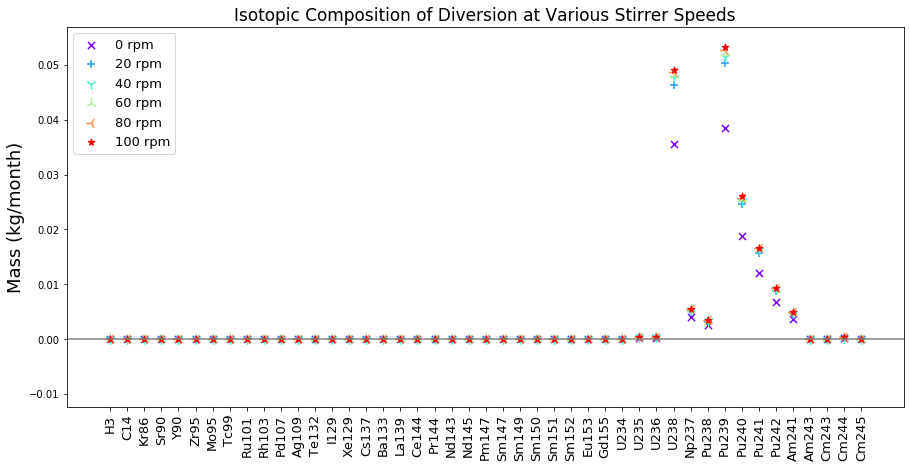
\includegraphics[width=\linewidth]{images/rotation-sa-comp}
	\caption{Isotopic composition of the diverted material stream at various central stirrer speeds.}
	\label{fig:ref-rot-sa}
\end{figure}

\begin{figure}
	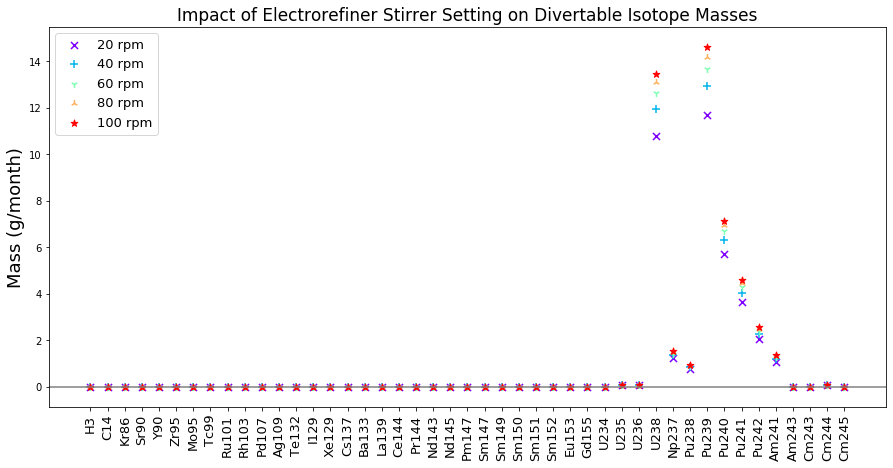
\includegraphics[width=\linewidth]{images/rotation-sa-diff}
	\caption{Isotopic composition of the diverted material stream at various central stirrer speeds.}
	\label{fig:ref-rot-diff}
\end{figure}

\subsection{Electrowinner Current}

The primary setting for the electrowinning sub-process is the current. The current's relationship with efficiency decreases in separation beginning around 10 A.
This is seen in Figures \ref{fig:win-cur-sa} and \ref{fig:win-cur-diff} as 10 A is below the efficiency of 5 A. This relationship occurs due to increasing voltage no longer aiding in separation of some lanthanides as described in chapter 2. Figure \ref{fig:win-cur-diff} shows that the key operating range lies within 6-8 A.

\begin{figure}
	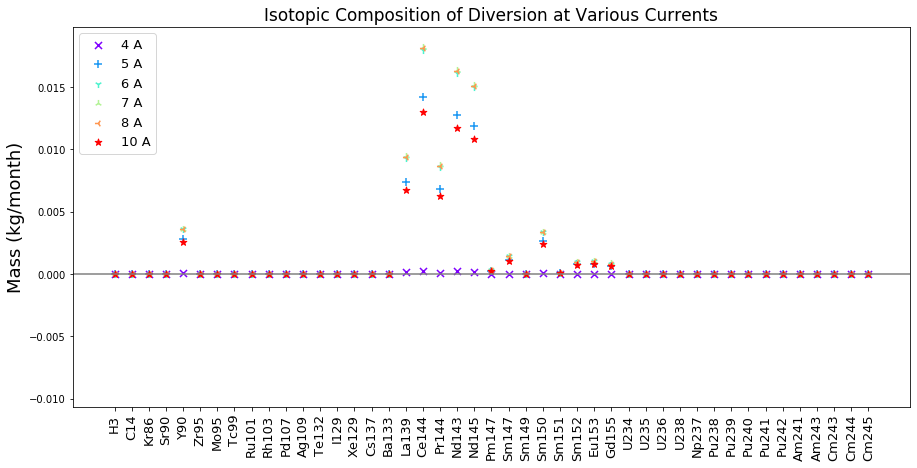
\includegraphics[width=\linewidth]{images/current-sa-comp}
	\caption{Isotopic composition of the diverted material stream at various electrowinner currents.}
	\label{fig:win-cur-sa}
\end{figure}

\begin{figure}
	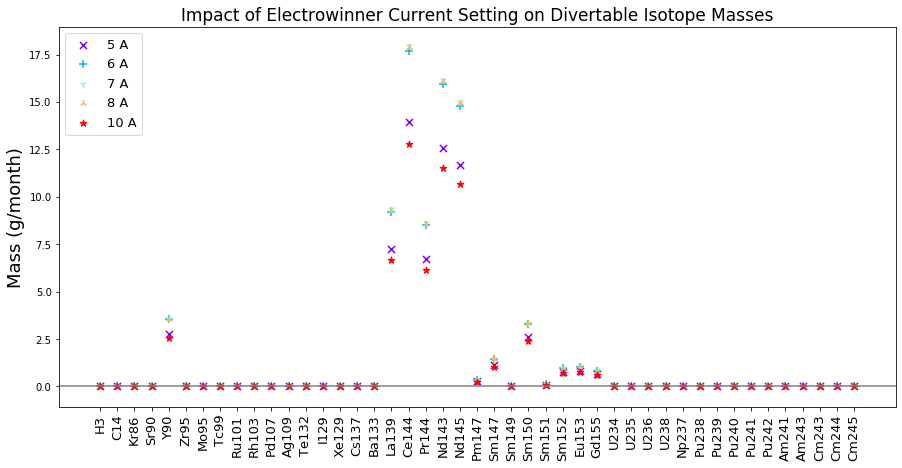
\includegraphics[width=\linewidth]{images/current-sa-diff}
	\caption{Isotopic composition of the diverted material stream at various electrowinner currents.}
	\label{fig:win-cur-diff}
\end{figure}

\subsection{Electrowinner Flow rate}

Similar to the central stirrer of the electrorefiner, increasing the flow rate through the electrowinner can aid removal of additional lanthanides and TRU. Flow rates shown are linear rates, with the bounds corresponding to minimum and maximum values tested in experimental facilities. Figures \ref{fig:win-flow-sa} and \ref{fig:win-flow-diff} demonstrate a steady increase in removal rates with increasing flow.

\begin{figure}
	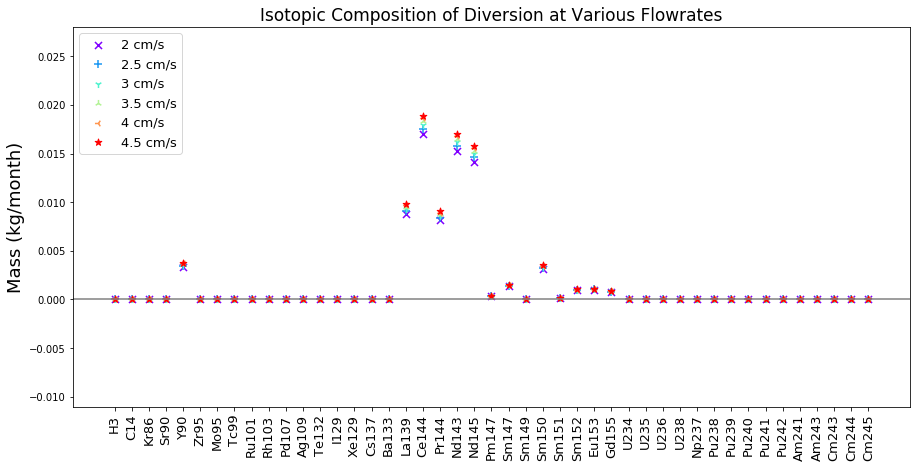
\includegraphics[width=\linewidth]{images/flowrate-sa-comp}
	\caption{Isotopic composition of the diverted material stream at various electrowinner flowrates.}
	\label{fig:win-flow-sa}
\end{figure}

\begin{figure}
	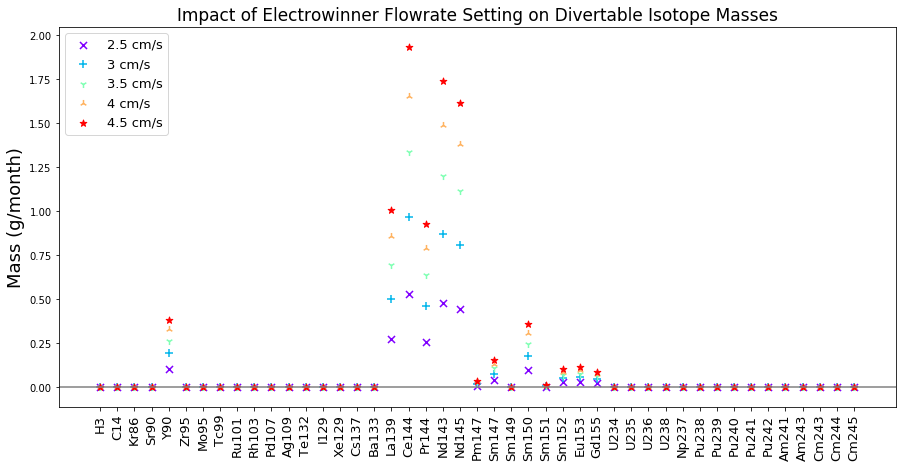
\includegraphics[width=\linewidth]{images/flowrate-sa-diff}
	\caption{Isotopic composition of the diverted material stream at various electrowinner flowrates.}
	\label{fig:win-flow-diff}
\end{figure}

\subsection{Electrowinner Reprocessing Time}

The final setting we chose to observe was time spent in the electrowinner. We chose this sub-process since it is closely related to the U/TRU product stream. Comparing Figure \ref{fig:win-time-diff} to Figure \ref{fig:win-flow-diff}, we can see that increasing 
reprocessing time results in more divertable material. 

\begin{figure}
	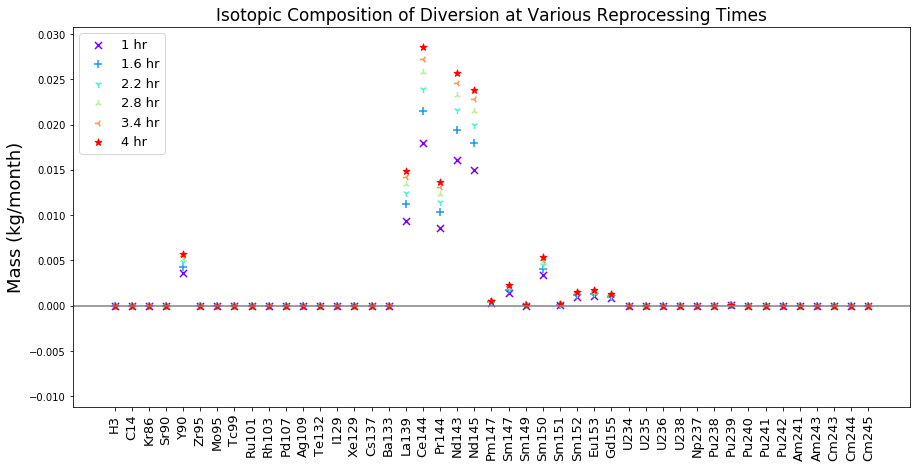
\includegraphics[width=\linewidth]{images/time-sa-comp}
	\caption{Isotopic composition of the diverted material stream at various electrowinner reprocessing durations.}
	\label{fig:win-time-sa}
\end{figure}

\begin{figure}
	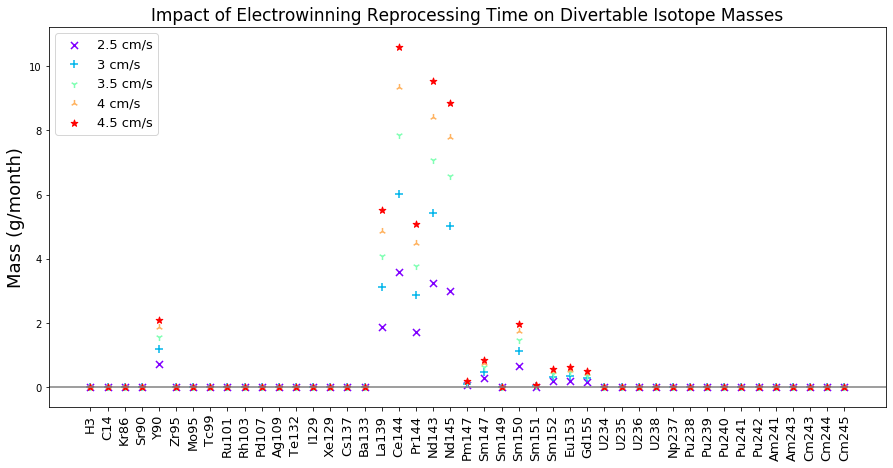
\includegraphics[width=\linewidth]{images/time-sa-diff}
	\caption{Isotopic composition of the diverted material stream at various electrowinner reprocessing durations.}
	\label{fig:win-time-diff}
\end{figure}

\section{Parameter Comparison}

The material increase due to the previous six operational settings was normalized against their respective baseline
to determine the most impactful process parameters. Table \ref{tab:compare} summarizes these values.

\begin{table}[h]
	\centering
	\begin{tabularx}{0.9\linewidth}{lcccccc}
		\hline
		\textbf{Sample} & \textbf{ER} & \textbf{ER} & \textbf{ER} & \textbf{EW}
		& \textbf{EW} & \textbf{EW} \\
		& \textbf{Temp} & \textbf{Pressure} & \textbf{Stir Speed} & \textbf{Current} & \textbf{Flow rate} & \textbf{Time} \\
		\hline \hline
		1 & 0.036 & 8.589 & 30.284 & 5.684 & 3.136 & 20.030 \\ \hline
		2 & 0.715 & 13.336 & 33.542 & 7.216 & 5.699 & 33.602 \\ \hline
		3 & 0.975 & 15.393 & 35.447 & 7.308 & 7.866 & 43.879 \\ \hline
		4 & 1.672 & 15.912 & 36.799 & 7.281 & 9.743 & 52.154 \\ \hline
		5 & 3.328 & 16.047 & 37.848 & 5.202 & 11.398 & 59.080 \\ \hline
	\end{tabularx}
	\caption {Comparison of operational settings' impact on divertable material (shown in
		\% difference compared to baseline values). Where ER and EW represent electrorefiner and electrowinner respectively.}
	\label {tab:compare}
\end{table}

Sensitivity analysis for each setting is split into corresponding samples to reflect increasing efficiency. As we observed earlier, temperature and current, although primary settings, 
do not result in significant increase in separated material. Temperature alterations result in diminishing returns, as a drastic increase of heat is required for noticeably improved efficiency. Notably,
the most impactful electrorefiner setting is the central stirrer's speed. The stirrer  
has such a significant impact due to increasing the rate of separation, and improving overall
efficiency. Comparing the stirrer and pressure separation efficiency illuminates the stirrer's significance. Reducing pressure to 100 mTorr results in a 16\% increase in material while a stirrer at 20 rpm nearly doubles that at 30.284\% increase.
Separation efficiency due to changes in current plateaus because the process is limited by reaction rate. Increasing electrowinner current does not affect opportunity to react as flowrate and time can be seen to do. 
A trend noticed in these settings is those which allow more interaction between the salt and waste see a more significant increase in product. 

While the rest also result in
improved efficiency, they require a larger change in operation to meet the same increased separation.